% Figure 1 (fig:overview) — TikZ source. This file is \input by
% sections/03_methodology.tex inside the figure* environment; iterate HERE.
%
% v3 (Robert's notes, 2026-07-13):
%   - Real street-map background (SZ_street_background_5x4_rotated.png, 5:4 =
%     the 10x8 panel exactly) under every panel; the synthetic TikZ roads are
%     gone. The district boundary is re-quantized to hug the map's wide
%     road corridor (top x~4 down to bottom x~7).
%   - Panel 3: SAME cell size as panels 1-2 (step=1); the *map* is zoomed 2x
%     (clipped to the image's lower-right quadrant) so the district boundary
%     sits at the left; longer trajectory with visible per-state dots, four
%     tail states per branch; more taxi squares; heat cells sized to the grid.
%   - Zoom box + "panel 3" cue removed (read as clutter).
%   - Legend value icon = three-step opacity gradient, flush with line icons.
%   - Bigger arrowheads throughout.
%   Two-hue scheme confirmed by Robert: vermillion = trim, blue = lift/supply.
%
% COLOR SYSTEM (2026-07-20, external design review; shared with fig-1):
%   hues muted — amber #D97706 = trim/excess/source, cobalt #2563EB =
%   lift/added; charcoal #4B5563 neutrals. Regional tints over the map:
%   pale amber ~10% = over-served, pale blue ~7% = under-served (color is
%   reinforcement — boundary dash + glyphs still carry the split in
%   grayscale). Trim's vacated origins are now pale-amber glyphs ("service
%   taken from an excess location"); relocated pickups stay gray (trim is
%   NOT added service — only lift's destination pick is cobalt).
%
% Geometry: 1 cell = 1 unit = 4.9mm; panel = 10x8 cells = 49mm x 39.2mm (the
% \includegraphics sizes below must track any unit change). Panel 3 shows the
% image's lower-right quadrant at 2x via clip + oversized include anchored at
% (-10,0). No \resizebox: fonts are true manuscript size.
\definecolor{figink}{HTML}{4B5563}
\definecolor{figgray}{HTML}{6B7280}
\definecolor{figfaint}{HTML}{D1D5DB}
\definecolor{figaccent}{HTML}{2563EB}
\definecolor{figtrim}{HTML}{D97706}
\begin{tikzpicture}[x=4.9mm, y=4.9mm, line cap=round, line join=round,
  % cell-scale marks: \pic[color=<c>] at (cell center) {pick};
  % service pickup: passenger stick figure (per Dr. Zhang 2026-07-18; was an x)
  pick/.pic={\draw[line width=0.8pt] (0,0.165) circle[radius=0.09];
             \draw[line width=0.8pt] (0,0.075) -- (0,-0.10);
             \draw[line width=0.8pt] (-0.14,0.005) -- (0.14,0.005);
             \draw[line width=0.8pt] (0,-0.10) -- (-0.12,-0.26)
                                     (0,-0.10) -- (0.12,-0.26);},
  % taxi presence: car glyph, body + cabin + wheels (was an open square)
  taxi/.pic={\draw[figink, fill=white, line width=0.7pt]
             (-0.27,-0.115) -- (-0.27,0.02) -- (-0.135,0.02)
             -- (-0.08,0.15) -- (0.12,0.15) -- (0.175,0.02)
             -- (0.27,0.02) -- (0.27,-0.115) -- cycle;
             \draw[figink, fill=white, line width=0.6pt]
             (-0.15,-0.115) circle[radius=0.06]
             (0.15,-0.115) circle[radius=0.06];},
  trimedit/.style={-{Stealth[length=5.5pt, width=4.5pt]}, figtrim,
                   line width=1.1pt},
  liftdash/.style={figaccent, dashed, line width=1.1pt},
  boundary/.style={figink!65, line width=1pt, dash pattern=on 4pt off 2pt},
  panelframe/.style={figgray, line width=0.6pt},
  citygrid/.style={figfaint, line width=0.4pt},
  % white translucent backing so labels stay readable over the map
  lbl/.style={fill=white, fill opacity=0.78, text opacity=1,
              inner sep=1.2pt, rounded corners=1pt}]

  % =========================================================================
  % Panel 1: the service gap  (full city)
  % =========================================================================
  \begin{scope}
    \node[anchor=south west, inner sep=0pt] at (0,0)
      {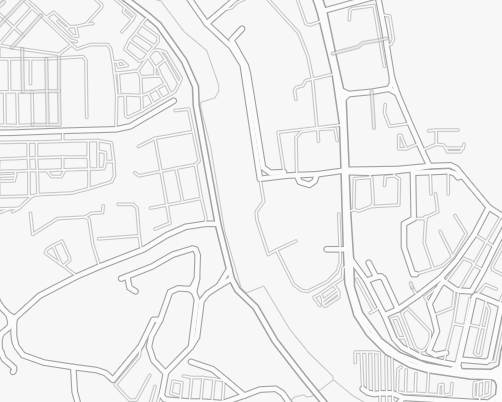
\includegraphics[width=49mm, height=39.2mm]{figures/figure-2/SZ_street_background_5x4_rotated}};
    % regional tints over the map: over-served pale amber, under-served
    % pale blue (translucent so the streets stay visible)
    \fill[figtrim, opacity=0.10] (0,0) -- (0,8) -- (4,8) -- (4,5) -- (5,5)
      -- (5,3) -- (6,3) -- (6,1) -- (7,1) -- (7,0) -- cycle;
    \fill[figaccent, opacity=0.07] (4,8) -- (4,5) -- (5,5) -- (5,3) -- (6,3)
      -- (6,1) -- (7,1) -- (7,0) -- (10,0) -- (10,8) -- cycle;
    \draw[citygrid, step=1] (0,0) grid (10,8);
    \draw[boundary] (4,8) -- (4,5) -- (5,5) -- (5,3) -- (6,3) -- (6,1)
      -- (7,1) -- (7,0);
    \draw[panelframe] (0,0) rectangle (10,8);
    % "locate the deficit" = §3.3's language (Attribution: Localizing the
    % Deficit...); parallel to panels (2)/(3): verb phrase after the colon
    \node[anchor=south west, font=\footnotesize, text=figink] at (0,8.2)
      {(1) Attribute: locate the deficit};
    % \node[anchor=south west, font=\footnotesize, text=figink] at (0,8.2)
    %   {(1) The service gap};
    % advantaged district: dense presence (cell-snapped), few pickups
    \foreach \x/\y in {1.5/6.5, 2.5/6.5, 3.5/6.5, 1.5/5.5, 3.5/5.5,
                       1.5/4.5, 2.5/4.5, 3.5/4.5, 2.5/7.5, 0.5/5.5}
      \pic at (\x,\y) {taxi};
    \foreach \x/\y in {2.5/5.5, 0.5/6.5, 0.5/4.5, 3.5/7.5}
      \pic[color=figgray] at (\x,\y) {pick};
    % disadvantaged district: dense unmet pickups, one taxi
    \foreach \x/\y in {8.5/1.5, 7.5/1.5, 8.5/2.5, 9.5/1.5, 7.5/0.5,
                       8.5/3.5, 9.5/2.5, 9.5/3.5}
      \pic[color=figgray] at (\x,\y) {pick};
    \pic at (7.5,2.5) {taxi};
    % district + service labels
    \node[lbl, font=\tiny, text=figink, align=center] at (2.1,3.3)
      {advantaged district\\(over-served)};
    \node[lbl, font=\tiny, text=figink, align=center] at (8.2,4.9)
      {disadvantaged district\\(under-served)};
    % legend (lower left)
    \fill[white, opacity=0.78, rounded corners=1pt]
      (0.12,0.08) rectangle (3.6,1.45);
    \pic at (0.5,1.05) {taxi};
    \node[anchor=west, font=\tiny, text=figink] at (0.85,1.05) {taxi presence};
    \pic[color=figgray] at (0.5,0.4) {pick};
    \node[anchor=west, font=\tiny, text=figink] at (0.85,0.4) {service pickup};
  \end{scope}

  % =========================================================================
  % Panel 2: trim  (same city; two pickups relocated inside the district)
  % =========================================================================
  \begin{scope}[shift={(11.5,0)}]
    \node[anchor=south west, inner sep=0pt] at (0,0)
      {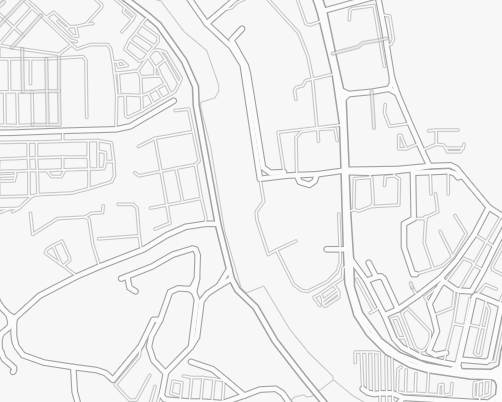
\includegraphics[width=49mm, height=39.2mm]{figures/figure-2/SZ_street_background_5x4_rotated}};
    \fill[figtrim, opacity=0.10] (0,0) -- (0,8) -- (4,8) -- (4,5) -- (5,5)
      -- (5,3) -- (6,3) -- (6,1) -- (7,1) -- (7,0) -- cycle;
    \fill[figaccent, opacity=0.07] (4,8) -- (4,5) -- (5,5) -- (5,3) -- (6,3)
      -- (6,1) -- (7,1) -- (7,0) -- (10,0) -- (10,8) -- cycle;
    \draw[citygrid, step=1] (0,0) grid (10,8);
    \draw[boundary] (4,8) -- (4,5) -- (5,5) -- (5,3) -- (6,3) -- (6,1)
      -- (7,1) -- (7,0);
    \draw[panelframe] (0,0) rectangle (10,8);
    \node[anchor=south west, font=\footnotesize, text=figink] at (0,8.2)
      {(2) Trim: relocate excess pickups};
    % same taxis; the two unedited pickups stay put
    \foreach \x/\y in {1.5/6.5, 2.5/6.5, 3.5/6.5, 1.5/5.5, 3.5/5.5,
                       1.5/4.5, 2.5/4.5, 3.5/4.5, 2.5/7.5, 0.5/5.5}
      \pic at (\x,\y) {taxi};
    \foreach \x/\y in {0.5/6.5, 3.5/7.5}
      \pic[color=figgray] at (\x,\y) {pick};
    % untouched disadvantaged district — identical to Panel 1
    \foreach \x/\y in {8.5/1.5, 7.5/1.5, 8.5/2.5, 9.5/1.5, 7.5/0.5,
                       8.5/3.5, 9.5/2.5, 9.5/3.5}
      \pic[color=figgray] at (\x,\y) {pick};
    \pic at (7.5,2.5) {taxi};
    % two trim edits: vacated origin (pale amber = service taken from an
    % excess location) -> amber arrow -> relocated pickup (gray: trim is
    % NOT added service), both inside the advantaged district
    \pic[color=figtrim!50] at (2.5,5.5) {pick};
    \draw[trimedit] (2.5,5.5) -- (4.5,4.5);
    \pic[color=figgray] at (4.5,4.5) {pick};
    \pic[color=figtrim!50] at (0.5,4.5) {pick};
    \draw[trimedit] (0.5,4.5) -- (1.5,3.5);
    \pic[color=figgray] at (1.5,3.5) {pick};
    \node[lbl, font=\tiny, text=figgray, align=center] at (8.0,6.9)
      {gap closes from the top:\\under-served untouched};
    % legend (lower left)
    \fill[white, opacity=0.78, rounded corners=1pt]
      (0.12,0.08) rectangle (6.0,1.45);
    \pic[color=figtrim!50] at (0.5,1.05) {pick};
    \node[anchor=west, font=\tiny, text=figink] at (0.85,1.05)
      {original position (vacated)};
    \draw[trimedit] (0.25,0.4) -- (0.8,0.4);
    \node[anchor=west, font=\tiny, text=figink] at (0.85,0.4)
      {trim edit (pickup relocated)};
  \end{scope}

  % =========================================================================
  % Panel 3: lift  (map zoomed 2x to the image's lower-right quadrant; grid
  % cells the SAME size as panels 1-2; district boundary off to the left)
  % =========================================================================
  \begin{scope}[shift={(23,0)}]
    \begin{scope}
      \clip (0,0) rectangle (10,8);
      % 2x map anchored so the visible window is the lower-right quadrant
      \node[anchor=south west, inner sep=0pt] at (-10,0)
        {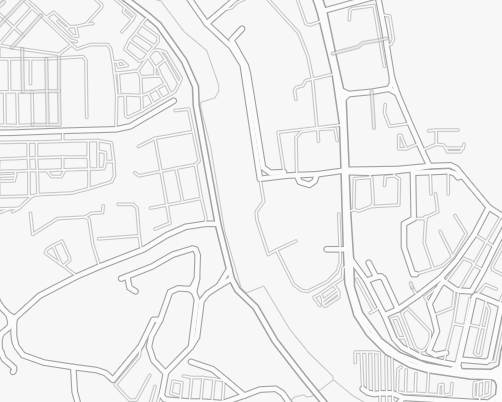
\includegraphics[width=98mm, height=78.4mm]{figures/figure-2/SZ_street_background_5x4_rotated}};
    \end{scope}
    % under-served district: everything east of the boundary (left sliver is
    % the advantaged edge, continuing the panels-1-2 corridor at 2x);
    % base tint kept lighter here so the value-of-presence field stays the
    % dominant blue signal
    \fill[figtrim, opacity=0.10] (0,0) -- (0,6) -- (2,6) -- (2,2) -- (4,2)
      -- (4,0) -- cycle;
    \fill[figaccent, opacity=0.05] (0,8) -- (0,6) -- (2,6) -- (2,2) -- (4,2)
      -- (4,0) -- (10,0) -- (10,8) -- cycle;
    % QUANTIZED value-of-presence field (accent cells, opacity = value)
    \fill[figaccent, fill opacity=0.26] (7,2) rectangle (8,3);   % peak
    \foreach \xa/\ya in {6/2, 8/2, 7/1, 7/3}
      \fill[figaccent, fill opacity=0.15] (\xa,\ya) rectangle (\xa+1,\ya+1);
    \foreach \xa/\ya in {6/1, 8/1, 6/3, 8/3}
      \fill[figaccent, fill opacity=0.07] (\xa,\ya) rectangle (\xa+1,\ya+1);
    \draw[citygrid, step=1] (0,0) grid (10,8);
    \draw[boundary] (0,6) -- (2,6) -- (2,2) -- (4,2) -- (4,0);
    \draw[panelframe] (0,0) rectangle (10,8);
    \node[anchor=south west, font=\footnotesize, text=figink] at (0,8.2)
      {(3) Lift: reroute seeking tails};
    \node[lbl, anchor=south west, font=\tiny, text=figgray] at (0.2,0.22)
      {under-served district (detail)};
    % recorded marks: dense unmet pickups, sparse taxi presence
    \foreach \x/\y in {6.5/2.5, 7.5/1.5, 8.5/2.5, 6.5/1.5, 8.5/3.5,
                       9.5/1.5, 5.5/0.5, 9.5/4.5}
      \pic[color=figgray] at (\x,\y) {pick};
    % (9.5,5.5) -> (8.5,4.5) 2026-07-20: cleared out from under the legend
    % box, which grew a line for the wrapped "value of added presence"
    \foreach \x/\y in {0.5/4.5, 1.5/2.5, 4.5/6.5, 8.5/4.5, 5.5/5.5}
      \pic at (\x,\y) {taxi};
    % one trajectory, two futures. Solid ink approach (per-state dots) to the
    % anchor; original tail (solid gray) reaches its recorded pickup; the
    % lift reroute (dashed accent) bends into the highest-value cell.
    \draw[figink, line width=1.2pt] (0.6,7.6) -- (1.3,6.9) -- (1.9,6.1)
      -- (2.4,5.3) -- (2.9,4.5) -- (3.4,3.8);
    \foreach \x/\y in {0.6/7.6, 1.3/6.9, 1.9/6.1, 2.4/5.3, 2.9/4.5, 3.4/3.8}
      \fill[figink] (\x,\y) circle (0.09);
    \draw[figgray, line width=1pt] (3.4,3.8) -- (3.9,3.1) -- (4.4,2.3)
      -- (5.0,1.5) -- (5.5,0.5);
    \foreach \x/\y in {3.9/3.1, 4.4/2.3, 5.0/1.5}
      \fill[figgray] (\x,\y) circle (0.09);
    \pic[color=figgray] at (5.5,0.5) {pick};
    \draw[liftdash] (3.4,3.8) -- (4.1,3.4) -- (5.0,3.0) -- (6.2,2.7);
    \draw[liftdash, -{Stealth[length=6pt, width=5pt]}] (6.2,2.7) -- (7.5,2.5);
    \foreach \x/\y in {4.1/3.4, 5.0/3.0, 6.2/2.7}
      \fill[figaccent] (\x,\y) circle (0.09);
    \pic[color=figaccent] at (7.5,2.5) {pick};
    % legend (upper right; bottom extended for the two-line third entry)
    \fill[white, opacity=0.78, rounded corners=1pt]
      (5.85,5.45) rectangle (9.95,7.85);
    \draw[figgray, line width=1pt] (6.1,7.5) -- (7.0,7.5);
    \node[anchor=west, font=\tiny, text=figink] at (7.15,7.5)
      {original tail};
    \draw[liftdash, -{Stealth[length=4.5pt, width=3.8pt]}]
      (6.1,6.9) -- (7.0,6.9);
    \node[anchor=west, font=\tiny, text=figink] at (7.15,6.9)
      {rerouted tail (lift)};
    % three-step opacity gradient icon, centered on the two-line label
    \fill[figaccent, fill opacity=0.07] (6.10,5.97) rectangle (6.38,6.33);
    \fill[figaccent, fill opacity=0.15] (6.41,5.97) rectangle (6.69,6.33);
    \fill[figaccent, fill opacity=0.26] (6.72,5.97) rectangle (7.00,6.33);
    \node[anchor=west, font=\tiny, text=figink, align=left] at (7.15,6.15)
      {value of added\\presence};
  \end{scope}
\end{tikzpicture}
